\section{Preliminary baseline results}

In initial prompt calibration, local Qwen3.5-0.8B assigned 9/10 and an empty issue list to all 18 pilot transcripts. The response-format example contained the score 9. After we removed the numeric example, this model flagged three injected claims and assigned 8/10 to every transcript.

We then ran J1 and J3 locally using the same Qwen3.5-9B model (Q4\_K\_M quantization) in llama.cpp, with thinking disabled and temperature zero. Under the pilot labeling rule, both protocols flagged the injected route error in all 15 variants. J1 lowered the score in five cases, left it unchanged in seven, and raised it in three. All five decreases came from the one original that J1 scored 9/10. The other two originals each scored 2/10, leaving only one point of downward room.

J3 gave all 15 edited dialogues a lower minimum score than their originals, and 14 reached the 1/10 floor. Across positions, the mean drops ranged from 6.00 to 6.33 points for J3 and from $-0.33$ to 2.33 for J1 (Figure~\ref{fig:positions}). J1 took 18 inference requests. J3 produced 186 turn scores from 114 distinct transcript prefixes, reusing outputs for identical inputs.

\paragraph{Aggregation sensitivity.}
Across all 15 pairs, the mean score drop was 6.27 points when we took the minimum turn score. Taking the mean over the same saved turn scores yielded a 2.32-point drop. Both aggregations gave a lower score to all 15 edited dialogues. The choice of rule therefore changed the size of the penalty even with identical turn judgments. In the Norwich 75\% variant, J3 gave the edited reply 2/10. The dialogue minimum of 1/10 came from a later, untouched reply because the judge revisited the restaurant details.

\paragraph{Audit of original judgments.}
The judges saw transcript text only. We checked three factual criticisms against the archived MultiWOZ records. In the Cambridge-to-Peterborough original (PMUL1801), J1 caught the typo \textit{Gald} and questioned the fare. The bundled record for train TR1086 gives \pounds13.20 per ticket, which verifies the quoted \pounds92.40 for seven. J1 flagged the Ely substitution in the early edit and gave both versions 2/10.

In the Norwich-to-Cambridge original (PMUL0509), the address and phone match Frankie and Bennys record 19195. J1 gave the dialogue 2/10 and reported an alleged mismatch as its sole issue. In the London-to-Cambridge original (MUL1569), the restaurant database has no South Indian entry. J3 nonetheless gave the reply reporting this result 2/10 and the other ten replies 10/10. The mistaken 2/10 set the dialogue score. Pre-existing flaws, factual false alarms, and scoring headroom all influence the paired scores.

\begin{figure}[t]
  \centering
  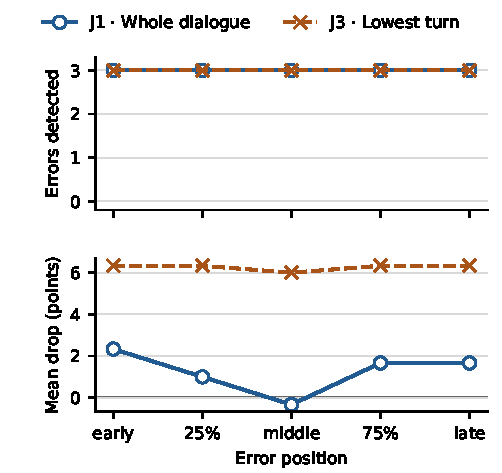
\includegraphics[width=\columnwidth]{position-curve.pdf}
  \caption{Qwen3.5-9B feasibility pilot across five assistant reply positions, with three edited dialogues per position. Detection uses the original pilot labeling rule. Score drops are paired differences from the unedited counterparts on the 1--10 scale.}
  \label{fig:positions}
\end{figure}
